\section{Evaluación y resultados}

En esta sección se explicarán las metodologías utilizadas para 
evaluar la solución y los principales resultados obtenidos.

%Comentarios de tincho:
% A quien se le hizo el test (muestra)
% Correlación
% Resumen de todo
% Encuesta objetiva
% Explicar a quien se le hizo el test, resumen, correlación
%3 paginas
\subsection{Encuesta para determinar la muestra}
\label{encuesta_muestra}
Para seleccionar a la muestra que participará en la evaluación de 
la versión final de la solución se realizó una encuesta con la que 
se determinó el nivel de acceso a la tecnología de los estudiantes 
del cuarto año de licenciatura en enfermería del IAB, además del 
tipo de acceso a internet, tipo de sistema operativo de sus teléfonos móviles 
y si cumplían con los requisitos técnicos para utilizar la solución. Estos 
requisitos son los siguientes:  memoria ram de $512$MB o superior, velocidad 
de procesador de $800$ GHz o superior y GPU Mali 400 o superior. 

La encuesta fue realizada a $124$ alumnos, se presentan a continuación los resultados.

\begin{figure}[H]
\centering
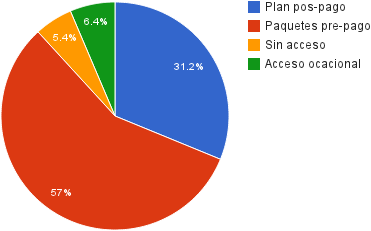
\includegraphics[scale=0.5]{../resultados/imagenes/ubicacion_acceso_internet.png}
\caption{Acceso a internet desde dispositivos móviles}
\label{fig:ubicacion_acceso_internet}
\end{figure}

\begin{figure}[H]
\centering
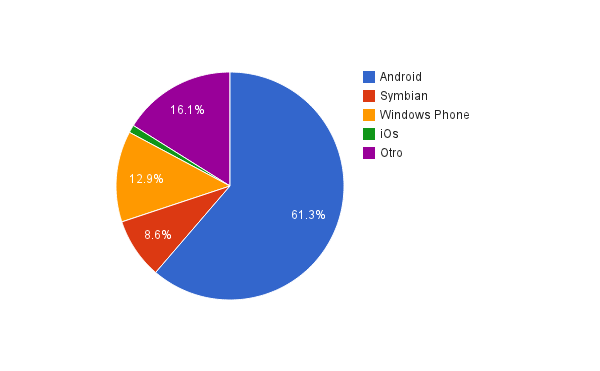
\includegraphics[scale=0.5]{../resultados/imagenes/ubicacion_sistemas_operativos.png}
\caption{Sistemas operativos móviles utilizados}
\label{fig:ubicacion_sistemas_operativos}
\end{figure}

\begin{figure}[H]
\centering
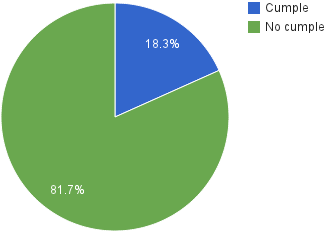
\includegraphics[scale=0.5]{../resultados/imagenes/ubicacion_requisitos_minimos.png}
\caption{Dispositivos que cumplen con los requisitos mínimos para la prueba}
\label{fig:ubicacion_requisitos_minimos}
\end{figure}

Del $18.3\%$ de los que cumplían con los requisitos, 11 alumnos estuvieron 
dispuestos a evaluar la solución. La utilización de $11$ alumnos es suficiente, ya que según estudios presentados
en~\cite{nielsen2000}, mientras menos experiencia tengan los sujetos de estudio
con la solución planteada, serán necesarios menos para detectar un gran
porcentaje de errores y fortalezas, y según~\cite{ritch2009}, una base de $10$ a
$12$ es suficiente para obtener resultados estadísticamente válidos.

\subsection{Encuesta para evaluar la solución}
\label{encuesta_solucion}
Con esta encuesta se busca identificar las fortalezas y debilidades de la 
solución, además de evaluar la solución en cuanto a factores de exploración, 
representación, motivación, inmersión, retroalimentación y pedagogía, de 
acuerdo a las apreciaciones de los miembros de la muestra. Además del nivel 
de aceptación de la solución por parte de ellos y la validación de las 
hipótesis planteadas como parte del desarrollo de la solución.

Las preguntas están agrupadas en dos, el primer grupo cuenta con $27$ 
preguntas cerradas, es decir de una sola respuesta en una lista de opciones, 
el segundo grupo cuenta con $4$ preguntas abiertas, es decir los encuestados 
pueden dar respuestas libres a las preguntas. 

En las preguntas cerradas la métrica utilizada es la escala de Likert
\cite{Allen:2007} de 7 valores posibles cuyo valor más alto es
\enquote{Totalmente de acuerdo} y el más bajo es \enquote{Totalmente en 
desacuerdo}. Una vez valoradas y registradas todas las respuestas y con el 
objetivo de eliminar las tendencias en la forma en la que son completadas las
encuestas\cite{Fischer2010} se utiliza el método de \emph{Doble 
Estandarización} recomendado en~\cite{Pagolu2011}, el promedio estandarizado 
refleja los puntos fuertes y débiles como se observan en los resultados 
principales que son presentados a continuación. 

\begin{table}[H]
\centering
\caption{Aceptación por aspecto de la solución}
\begin{tabular}{lcr}
\toprule
Factores        & Promedio encuesta      & Promedio estandarizado \\
\midrule
Motivación               & De acuerdo              & $0.67$  \\
Facilidad de exploración & De acuerdo              & $0.68$  \\
Sensación de Inmersión   & De acuerdo              & $0.63$  \\
Pedagogía                & De acuerdo              & $0.67$  \\
Representación           & Parcialmente de acuerdo & $0.53$  \\
Retroalimentación        & Parcialmente de acuerdo & $0.60$  \\
Utilidad                 & De acuerdo              & $0.69$  \\
\bottomrule
\end{tabular}
\label{tab:resultado_resumen_aspectos_aceptacion}
\end{table}

\begin{table}[H]
\centering
\caption{Hipótesis con su aceptación}
\begin{tabular}{lcr}
\toprule
Hipótesis                        & Promedio encuesta     & Promedio estandarizado \\
\midrule
Comandos de voz con interfaz     & De acuerdo              & $0,55$ \\
Extracción uniforme de elementos & Parcialmente de acuerdo & $0,65$ \\
Acciones de bioseguridad         & De acuerdo              & $0,58$ \\
Representación iconográfica      & Parcialmente de acuerdo & $0,53$ \\
Factores motivadores             & De acuerdo              & $0,65$ \\
Falta de pistas                  & De acuerdo              & $0,61$ \\
\bottomrule
\end{tabular}

\label{tab:resultado_resumen_hipotesis}
\end{table}

\begin{figure}[H]
\centering
\begin{tikzpicture}[label distance=.15cm]
\tkzKiviatDiagram[radial=2,
                    lattice=2, step=2,
                    scale=1.5]%
                {Motivación,
                Facilidad de exploración,
                 Sensación de inmersión,
                 Pedagogía,
                 Representación,
                 Retroalimentación,
                 Utilidad}
\tkzKiviatLine[thick,
                color=blue,
                mark=ball,
                ball color=red,
                mark size=1pt,opacity=.2, 
                fill=red!20](0.67,0.68,0.63,0.67,0.53,0.60,0.69)
\end{tikzpicture}
\label{fig:subjetiva_kiviat}
\caption{Gráfico de Kiviat de los factores evaluados}
\end{figure}

\subsection{Encuesta para evaluar el conocimiento}
\label{encuesta_conocimiento}
A fin de obtener información acerca del conocimiento de los alumnos que 
utilizaron la solución propuesta y los que no la utilizaron, los cuales 
constituyen el grupo de control, se realiza una encuesta que consta de diez 
preguntas.

La encuesta mide el nivel de conocimiento del alumno sobre los dos temas 
simulados, contiene preguntas de nivel básico, medio y avanzado. Las mismas 
son formuladas utilizando la lista de competencias básicas que debe tener un 
alumno para aprobar la materia \textbf{Enfermería en Urgencias II}. Las 
preguntas son verificadas  por los profesores de la cátedra. Cada pregunta 
tiene el mismo peso, así la puntuación más baja obtenible es $0$, y la más 
alta es $10$.

De esta manera se busca evaluar la influencia pedagógica y la utilidad de la 
solución como herramienta de apoyo al aprendizaje. Dado que la cantidad de 
partidas jugadas por usuario por tipo de procedimiento no es considerada 
suficiente no se pueden considerar las diferencias entre la muestra y el 
grupo de control como absolutas. Cabe destacar que el objetivo principal es 
el de proveer una herramienta útil, la evaluación del nivel de aprendizaje 
es sólo para estimar su impacto en un nivel más alto. A continuación se 
muestra un resumen de los resultados.

\begin{table}[!hbt]
\centering
\caption{Rendimiento promedio de usuarios por pregunta}
\begin{tabular}{lrrr}
\toprule
\textbf{Pregunta} & 
\textbf{Prom. Muestra} & 
\textbf{Prom. Grupo Control} & 
\textbf{Prom. Total} \\ 
\midrule
1         & 0.36 & 0.18 & 0.20 \\
2         & 0.64 & 0.60 & 0.60 \\
3         & 0.09 & 0.14 & 0.13 \\
4         & 0.27 & 0.25 & 0.26 \\
5         & 0.82 & 0.56 & 0.59 \\
6         & 0.00 & 0.18 & 0.16 \\
7         & 0.64 & 0.51 & 0.53 \\
8         & 0.45 & 0.27 & 0.29 \\
9         & 0.18 & 0.32 & 0.31 \\
10        & 0.36 & 0.45 & 0.45 \\
\midrule
\textbf{Promedio}: & 3.82 & 3.47 & 3.49  \\
\bottomrule
\end{tabular}

\label{tab:objetiva_rendimiento_por_pregunta}
\end{table}

\subsection{Registro de actividades}

La solución propuesta almacena información relacionada a la actividad del
usuario, incluyendo cuando y como utiliza las acciones, los pasos que realiza,
el orden y las condiciones de la escena cuando realiza cada acción, el tiempo de
partida por procedimiento, entre otras informaciones.

El registro de actividades ayuda a identificar las  fortalezas y debilidades de
la solución en cuanto al diseño y utilidad. Sobre todo, ayuda a medir el impacto
pedagógico al permitir contrarrestar el uso y desempeño del usuario con el
puntaje obtenido por el mismo en la encuesta utilizada para medir el
conocimiento. EL principal resultado obtenido es la correlación de Pearson
\cite{BoslaughStatistics2008} entre los datos del registro de actividades y de
la encuesta de conocimiento considerando sólo a la muestra, a continuación se
muestran estos resultados.

\begin{table}[H]
\centering
\caption{Correlación entre factores estudiados} 
\begin{tabular}{lrrrrrr}
\toprule
        &
\begin{sideways}\textbf{Tiempo de Uso}\end{sideways}             &
\begin{sideways}\textbf{Encuesta subjetiva}\end{sideways}        &
\begin{sideways}\textbf{Encuesta objetiva}\end{sideways}         &
\begin{sideways}\textbf{Puntaje Máximo Extracción}\end{sideways} &
\begin{sideways}\textbf{Puntaje Máximo Glasgow}\end{sideways}    \\
\midrule
Tiempo de Uso             & 1    & -0.2  & 0.15  & 0.62 & 0.41 & 0.78 \\
Encuesta subjetiva        & -0.2 & 1     & -0.07 & 0.04 & 0.11 & -0.28\\
Encuesta objetiva         & 0.15 & -0.07 & 1     & 0.44 & 0.44 & 0.02 \\
Puntaje máximo Extracción & 0.62 & 0.04  & 0.44  & 1    & 0.96 & 0.44 \\
Puntaje máximo Glasgow    & 0.41 & 0.11  & 0.44  & 0.96 & 1    & 0.27 \\
\bottomrule               & 0.78 & -0.28 & 0.02  & 0.44 & 0.27 & 1    \\
\end{tabular}

\label{tab:all_correlation}
\end{table}

Las correlaciones fuertes, que se observan en la
tabla~\ref{tab:all_correlation}, son:

\begin{itemize}
    \item Tiempo de uso y puntaje máximo extracción, $0,62$, correlación
        positiva fuerte.
    \item Tiempo de uso y puntaje máximo Glasgow, $0,78$, correlación positiva
        muy fuerte.
    \item Puntaje máximo extracción y encuesta objetiva, $0,44$, correlación
        positiva fuerte.
\end{itemize}


%Los tres gráficos (estos gráficos son de la ubicación)
%\subsection{Variables}
%\subsection{Resultados}
%\begin{itemize}
%\item Aceptación de la solución (estrella de kiviat)
%\item Correlación
%\end{itemize}
